\documentclass{beamer}


%\usepackage{graphicx}
\usepackage{verbatim}

\useoutertheme{shadow}
%\usecolortheme{orchid}
\usecolortheme{seahorse}

\renewcommand{\a}{\alpha}
\renewcommand{\b}{\beta}
\renewcommand{\d}{\delta}
\newcommand{\g}{\gamma}
\newcommand{\s}{\sigma}
\newcommand{\w}{\omega}
\renewcommand{\k}{\vec{k}}
\newcommand{\td}[1]{\tilde{#1}}
\newcommand{\x}{\vec{x}}
\newcommand{\p}{\phantom{\alpha}}

\def\toonscale{0.45}
\def\mboxy#1{\mbox{\small #1}}


\begin{comment}
\AtBeginSection[]{
  \frame{
    \frametitle{Outline}
    \tableofcontents[currentsection]
  }
}
\end{comment}

\title{PTA Confusion}
\subtitle{Resolution, Source Confusion and Stochasticity in Pulsar Timing Arrays}
\author[Boyle and Pen]{Latham Boyle and Ue-Li Pen \\[8mm] 
}
\date{Max-Planck-Institut f\"ur Radioastronomie, 16. August, 2010}


\begin{document}

\frame{\titlepage}

%\section*{Introduction}
\section{Introduction}

\begin{comment}
  \subsection{Outline}

  \frame{
    \frametitle{Outline}
    \tableofcontents
  }
\end{comment}

  \subsection{PTA}
  \frame{
    \frametitle{Dectecting Gravity Waves}
    \begin{itemize}
	\item Theorist's picture: measure timing residuals along
          various lines of sights to pulsars      
	\item two modes: distance to pulsar known (3-D), or unknown
          (2-D)
        \item make 2-D or 3-D map of strain on the sky as a function
          of gravity wave period.
        \item extension of Boyle 2010 ``Porcupine'' detector formalism
          (mega-ligo) 
    \end{itemize}
  }

  \subsection{2-D}

  \frame{
    \frametitle{Background}
    \begin{itemize}
      \item traditional technique: measure 2 point correlation function of residuals (Jenet, etc).
      \item equivalent to power spectrum
      \item potentially very non-optimal for point sources -- c.f.
        hubble deep field.
      \item new ``imaging'' approach
      \item initial detections will be most sensitive for
        $\lambda_{\rm GW} \sim t_{\rm obs}$.  We will study this limit.
      \item start with the limit of a dense sample of pulsars, and ask
        what happens as density is reduced
      \item should reduce to previously known limits w.r.t. confusion
        (e.g. Sesana et al 2008)
    \end{itemize}
  }

\section{Gravity Wave Image}

\subsection{Residual}
\frame{
  \frametitle{Formulation}
TT gauge line element:
\begin{equation}
  \label{metric}
  ds^{2}=-dt^{2}+[\delta_{ij}+2h_{ij}]dx^{i}dx^{j}.
\end{equation}
In this gauge, the $\vec{x}={\rm constant}$ worldlines are timelike
geodesics; along such a worldline, the proper time $\tau$ is just the
coordinate time $t$.   Single gravitational
plane wave travelling in the $\hat{n}$ direction
\begin{equation}
  \label{deltat(omega)}
  \delta \tilde{t}_{\alpha}(\omega)=\frac{i}{\omega}
  \frac{\tilde{h}_{ij}(\omega)\hat{r}_{\alpha}^{i}\hat{r}_{\alpha}^{j}
    [1-{\cal P}_{\alpha}(\omega)]}{(1\!+\!\hat{n}\!\cdot\!\hat{r}_{\alpha})}
\end{equation}
with phase
\begin{equation}
  \label{P_alpha}
  {\cal P}_{\alpha}(\omega)\equiv
  {\rm e}^{i\omega r_{\alpha}(1+\hat{n}\cdot\hat{r}_{\alpha})}.
\end{equation}
reduces to $\delta t = \sin(2\phi)[1+\cos(\theta)]$ when averaging
over all pulsar distances.  Well known result.
}

  \subsection{E-M Analogue}

  \frame{
    \frametitle{Radio Interferometers}
    \begin{itemize}
      \item Measures electric field $E_i$, v.s. strain $h_{ij}$
      \item Transverse wave
      \item Image (radiation power) detection is quadratic in $E$ (or $h$)
      \item stationary in time, fourier modes
      \item Source power spectrum is quadratic in image, quartic in field.
    \end{itemize}
  }

  \frame{
    \frametitle{Residual Image}
%    \begin{minipage}{0.6\linewidth}
    \vspace{-0.2in}
    \begin{itemize}
    \item \mboxy{$\delta t = \sin(2\phi)[1+\cos(\theta)]$}
    \end{itemize}
%    \end{minipage}
    \begin{minipage}{0.35\linewidth}
      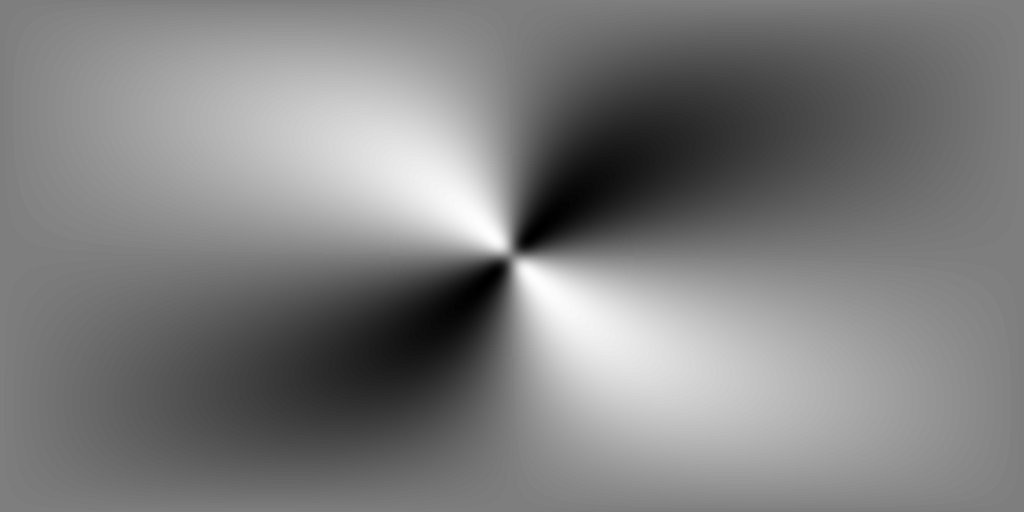
\includegraphics[scale=0.25]{residual}
    \end{minipage}
    \hspace{0.02\linewidth}
    
    
    singular spatial structure near GW source, no residual in
    anti-direction (TT).  
    }

  \frame{
    \frametitle{Two sources}
      \vspace{0.5cm}
      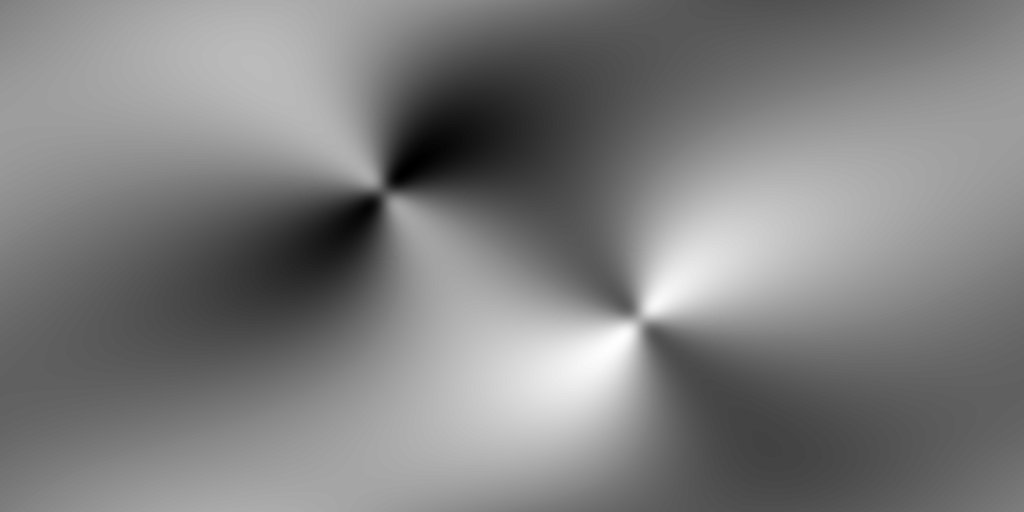
\includegraphics[scale=0.25]{residual2}
    \begin{itemize}
      \item Well resolved by dense PTA
    \end{itemize}
    }



  \subsection{Finite Corrections}

  \frame{
    \frametitle{Distance}
    \begin{itemize}
    \item At angles $\theta < \sqrt{\frac{\lambda_{\rm GW}}{r}}$ the
      intrinsic pulsar delay cancels the earth delay
    \item Typical distances $r \sim$ kpc, $\lambda_{\rm GW} \sim 3 $ pc,
      $\theta \sim 5^o$
    \item Confused if more than 100's of sources, or more sources than
      pulsars. 
    \end{itemize}
  }
      
  \frame{
    \frametitle{Sensitivity}
    \begin{itemize}
    \item 20 resolution pixels without loss of sensitivity:
    \item 5 quadrupoles, 2 polarizations, 2 front-back
    \item most models have resolvable brightest source with
      factor of 20 boost (Sesana et al 2008)
    \item stochastic  non-optimal
    \item with $> 20$ sources, resolvability relies on pulsars near
      the GW source 
    \item depends on luminosity distribution, etc
    \item only valid is $N_{\rm pulsar}>N_{\rm resolution}$
    \item Poisson model results in $\sim 2$ gain in sensitivity,
      depends on pulsar spatial and timing noise distribution.
    \end{itemize}
  }


  \subsection{Statistics}

  \frame{
    \frametitle{Forecasts}
    \begin{itemize}
    \item Jenet et al  measure the spatial 2-PCF of timing
      residuals at fixed wavelength
    \item $\xi(\theta)=\langle \delta t(0) \delta t(\theta) \rangle$
      fixed at single source $\theta=0$
    \item expectation value of $\langle \xi \rangle = \frac{3}{2} x \log x-\frac{x}{4}+\frac{1}{2}$, where $x=[1-\cos(\theta)]/2$
    \item erases the singular structures
    \item then weight $\int \xi \langle \xi \rangle dx$
    \item only optimal if average strain is 20 times larger than peak
      strain.
    \item factor of 20 was assumed to be order unity
    \item Instead, fit for individual source gravity wave templates
    \end{itemize}    
  }
  \frame{
    \frametitle{2-PCF}
    \begin{itemize}
    \item What went wrong with 2-PCF confusion analysis?
    \item in the map confused limit, 2-PCF is optimal.
    \item apply 2-PCF to test for confusion: concluded that it is
      source confused, and therefore optimal.
    \item Logic fails because confusion must hold at map/pixel level for
      2-PCF to be optimal.
    \item 2-PCF confusion does not imply map confusion!
    \item other sources of Gaussian non-optimality studied
      (e.g. Sasana and Vecchio 2010, van Haasteren 2009)
    \end{itemize}    
  }

  \section{3-D imaging}
  \subsection{GW interferometry}
  \frame{
    \frametitle{3-D}
    \begin{itemize}
      \item if distances to pulsars are known to better than 1
        wavelength, source positions are known to $\delta \theta \sim
        \frac{\lambda}{D}$.
      \item complications when pulsar period changes over the 3-D extent of PTA
    \end{itemize}
  }

  \frame{
    \frametitle{Distance measurement}
    \begin{itemize}
    \item direct parallax: current best VLBI pulsar distances to $\delta \alpha \sim 20 \mu$ sec. 
    \item need $\delta r = r \delta \alpha \frac{r}{r_{
          \rm AU}} < 3pc$
    \item current techniques accessible to $r \lesssim 200$ pc.
    \item limited by availability of bright nearby VLBI calibrators,
        flux, ionosphere, troposphere, etc.
      \item substantial improvements in principle possible with more
        sensitivity.  Perhaps $r \sim $kpc for SKA?
    \end{itemize}
  }
  \frame{
    \frametitle{Interferometric Self-cal}
    \begin{itemize}
    \item In radio interferometry, position of detectors can be solved
      from data.
    \item For single monochromatic source, distance to pulsar is
      degenerate modulo wavelength
    \item broken by multiple sources, and/or period change.
    \end{itemize}
  }

  \subsection{Conclusions}
  \frame{
    \frametitle{Conclusions}
    \begin{itemize}
    \item Confusion spatial resolution of 2-D PTA: $<$ 90 degrees for
      all cases, $< 5$ degrees for dense sampling. Timing residual map
      has rich spatial structure, which is erased in correlation
      function analysis.
    \item 3-D: $\sim \frac{10'}{\rm SNR}$
    \item Changes physical interpretation of PTA GW signals: unlikely
      to be in stochastic regime.  2-PCF confusion analysis is
      self-fulfilling prophecy.
    \item PTA has potential to be high resolution GW telescope
    \item motivation for precision pulsar VLBI paralax
    \item  cylinder transit surveys  may accelerate pulsar search
      (c.f. Kaspi, Ransom)
    \end{itemize}
  }
\end{document}
